% This file was converted to LaTeX by Writer2LaTeX ver. 1.4
% see http://writer2latex.sourceforge.net for more info
\documentclass[12pt]{article}
\usepackage[utf8]{inputenc}
\usepackage[T1]{fontenc}
\usepackage[english]{babel}
\usepackage{amsmath}
\usepackage{amssymb,amsfonts,textcomp}
\usepackage{array}
\usepackage{supertabular}
\usepackage{hhline}
\usepackage{hyperref}
\hypersetup{colorlinks=true, linkcolor=blue, citecolor=blue, filecolor=blue, urlcolor=blue}
\usepackage{graphicx}
% footnotes configuration
\makeatletter
\renewcommand\thefootnote{\arabic{footnote}}
\makeatother
% Text styles
\newcommand\textstyleInternetlink[1]{#1}
\newcommand\textstyleListLabelxix[1]{#1}
\newcommand\textstyleListLabelxx[1]{#1}
\newcommand\textstyleListLabelxxi[1]{#1}
\newcommand\textstyleListLabelxxii[1]{#1}
\makeatletter
\newcommand\arraybslash{\let\\\@arraycr}
\makeatother
\raggedbottom
% Paragraph styles
\renewcommand\familydefault{\rmdefault}
\newenvironment{styleStandard}{\setlength\leftskip{0cm}\setlength\rightskip{0cm plus 1fil}\setlength\parindent{0cm}\setlength\parfillskip{0pt plus 1fil}\setlength\parskip{0in plus 1pt}\writerlistparindent\writerlistleftskip\leavevmode\normalfont\normalsize\writerlistlabel\ignorespaces}{\unskip\vspace{0.111in plus 0.0111in}\par}
\newenvironment{stylelsSectioni}{\setlength\leftskip{0.25in}\setlength\rightskip{0in plus 1fil}\setlength\parindent{0in}\setlength\parfillskip{0pt plus 1fil}\setlength\parskip{0.1665in plus 0.016649999in}\writerlistparindent\writerlistleftskip\leavevmode\normalfont\normalsize\fontsize{18pt}{21.6pt}\selectfont\bfseries\writerlistlabel\ignorespaces}{\unskip\vspace{0.0835in plus 0.00835in}\par}
\newenvironment{stylelsSectionii}{\setlength\leftskip{0.25in}\setlength\rightskip{0in plus 1fil}\setlength\parindent{0in}\setlength\parfillskip{0pt plus 1fil}\setlength\parskip{0.222in plus 0.0222in}\writerlistparindent\writerlistleftskip\leavevmode\normalfont\normalsize\fontsize{16pt}{19.2pt}\selectfont\bfseries\writerlistlabel\ignorespaces}{\unskip\vspace{0.0835in plus 0.00835in}\par}
\newenvironment{stylecaption}{\setlength\leftskip{0cm}\setlength\rightskip{0cm plus 1fil}\setlength\parindent{0cm}\setlength\parfillskip{0pt plus 1fil}\setlength\parskip{0.0835in plus 0.00835in}\writerlistparindent\writerlistleftskip\leavevmode\normalfont\normalsize\fontsize{10pt}{12.0pt}\selectfont\itshape\writerlistlabel\ignorespaces}{\unskip\vspace{0.0835in plus 0.00835in}\par}
\newenvironment{styleListParagraph}{\setlength\leftskip{0.5in}\setlength\rightskip{0in plus 1fil}\setlength\parindent{0in}\setlength\parfillskip{0pt plus 1fil}\setlength\parskip{0in plus 1pt}\writerlistparindent\writerlistleftskip\leavevmode\normalfont\normalsize\writerlistlabel\ignorespaces}{\unskip\vspace{0.111in plus 0.0111in}\par}
% List styles
\newcommand\writerlistleftskip{}
\newcommand\writerlistparindent{}
\newcommand\writerlistlabel{}
\newcommand\writerlistremovelabel{\aftergroup\let\aftergroup\writerlistparindent\aftergroup\relax\aftergroup\let\aftergroup\writerlistlabel\aftergroup\relax}
\newcounter{listWWNumxxiileveli}
\newcounter{listWWNumxxiilevelii}[listWWNumxxiileveli]
\newcounter{listWWNumxxiileveliii}[listWWNumxxiilevelii]
\newcounter{listWWNumxxiileveliv}[listWWNumxxiileveliii]
\renewcommand\thelistWWNumxxiileveli{\arabic{listWWNumxxiileveli}}
\renewcommand\thelistWWNumxxiilevelii{\arabic{listWWNumxxiileveli}.\arabic{listWWNumxxiilevelii}}
\renewcommand\thelistWWNumxxiileveliii{\arabic{listWWNumxxiileveli}.\arabic{listWWNumxxiilevelii}.\arabic{listWWNumxxiileveliii}}
\renewcommand\thelistWWNumxxiileveliv{\arabic{listWWNumxxiileveli}.\arabic{listWWNumxxiilevelii}.\arabic{listWWNumxxiileveliii}.\arabic{listWWNumxxiileveliv}}
\newcommand\labellistWWNumxxiileveli{\thelistWWNumxxiileveli.}
\newcommand\labellistWWNumxxiilevelii{\thelistWWNumxxiilevelii.}
\newcommand\labellistWWNumxxiileveliii{\thelistWWNumxxiileveliii.}
\newcommand\labellistWWNumxxiileveliv{\thelistWWNumxxiileveliv.}
\newenvironment{listWWNumxxiileveli}{\def\writerlistleftskip{\setlength\leftskip{0.5in}}\def\writerlistparindent{}\def\writerlistlabel{}\def\item{\def\writerlistparindent{\setlength\parindent{-0.25in}}\def\writerlistlabel{\stepcounter{listWWNumxxiileveli}\makebox[0cm][l]{\labellistWWNumxxiileveli}\hspace{-0.635cm}\writerlistremovelabel}}}{}
\newenvironment{listWWNumxxiilevelii}{\def\writerlistleftskip{\setlength\leftskip{1in}}\def\writerlistparindent{}\def\writerlistlabel{}\def\item{\def\writerlistparindent{\setlength\parindent{-0.25in}}\def\writerlistlabel{\stepcounter{listWWNumxxiilevelii}\makebox[0cm][l]{\labellistWWNumxxiilevelii}\hspace{-1.905cm}\writerlistremovelabel}}}{}
\newenvironment{listWWNumxxiileveliii}{\def\writerlistleftskip{\setlength\leftskip{1.5in}}\def\writerlistparindent{}\def\writerlistlabel{}\def\item{\def\writerlistparindent{\setlength\parindent{-0.1252in}}\def\writerlistlabel{\stepcounter{listWWNumxxiileveliii}\makebox[0cm][r]{\labellistWWNumxxiileveliii}\hspace{-3.4919918cm}\writerlistremovelabel}}}{}
\newenvironment{listWWNumxxiileveliv}{\def\writerlistleftskip{\setlength\leftskip{2in}}\def\writerlistparindent{}\def\writerlistlabel{}\def\item{\def\writerlistparindent{\setlength\parindent{-0.25in}}\def\writerlistlabel{\stepcounter{listWWNumxxiileveliv}\makebox[0cm][l]{\labellistWWNumxxiileveliv}\hspace{-4.4449997cm}\writerlistremovelabel}}}{}
\newcounter{listWWNumxxivleveli}
\newcounter{listWWNumxxivlevelii}[listWWNumxxivleveli]
\newcounter{listWWNumxxivleveliii}[listWWNumxxivlevelii]
\newcounter{listWWNumxxivleveliv}[listWWNumxxivleveliii]
\renewcommand\thelistWWNumxxivleveli{\arabic{listWWNumxxivleveli}}
\renewcommand\thelistWWNumxxivlevelii{\alph{listWWNumxxivlevelii}}
\renewcommand\thelistWWNumxxivleveliii{\roman{listWWNumxxivleveliii}}
\renewcommand\thelistWWNumxxivleveliv{\arabic{listWWNumxxivleveliv}}
\newcommand\labellistWWNumxxivleveli{(\thelistWWNumxxivleveli)}
\newcommand\labellistWWNumxxivlevelii{\thelistWWNumxxivlevelii.}
\newcommand\labellistWWNumxxivleveliii{\thelistWWNumxxivleveliii.}
\newcommand\labellistWWNumxxivleveliv{\thelistWWNumxxivleveliv.}
\newenvironment{listWWNumxxivleveli}{\def\writerlistleftskip{\setlength\leftskip{0.5in}}\def\writerlistparindent{}\def\writerlistlabel{}\def\item{\def\writerlistparindent{\setlength\parindent{-0.25in}}\def\writerlistlabel{\stepcounter{listWWNumxxivleveli}\makebox[0cm][l]{\labellistWWNumxxivleveli}\hspace{-0.635cm}\writerlistremovelabel}}}{}
\newenvironment{listWWNumxxivlevelii}{\def\writerlistleftskip{\setlength\leftskip{1in}}\def\writerlistparindent{}\def\writerlistlabel{}\def\item{\def\writerlistparindent{\setlength\parindent{-0.25in}}\def\writerlistlabel{\stepcounter{listWWNumxxivlevelii}\makebox[0cm][l]{\labellistWWNumxxivlevelii}\hspace{-1.905cm}\writerlistremovelabel}}}{}
\newenvironment{listWWNumxxivleveliii}{\def\writerlistleftskip{\setlength\leftskip{1.5in}}\def\writerlistparindent{}\def\writerlistlabel{}\def\item{\def\writerlistparindent{\setlength\parindent{-0.1252in}}\def\writerlistlabel{\stepcounter{listWWNumxxivleveliii}\makebox[0cm][r]{\labellistWWNumxxivleveliii}\hspace{-3.4919918cm}\writerlistremovelabel}}}{}
\newenvironment{listWWNumxxivleveliv}{\def\writerlistleftskip{\setlength\leftskip{2in}}\def\writerlistparindent{}\def\writerlistlabel{}\def\item{\def\writerlistparindent{\setlength\parindent{-0.25in}}\def\writerlistlabel{\stepcounter{listWWNumxxivleveliv}\makebox[0cm][l]{\labellistWWNumxxivleveliv}\hspace{-4.4449997cm}\writerlistremovelabel}}}{}
\newcommand\labellistWWNumxxxvleveli{\textstyleListLabelxix{[F0B7?]}}
\newcommand\labellistWWNumxxxvlevelii{\textstyleListLabelxx{o}}
\newcommand\labellistWWNumxxxvleveliii{\textstyleListLabelxxi{[F0A7?]}}
\newcommand\labellistWWNumxxxvleveliv{\textstyleListLabelxxii{[F0B7?]}}
\newenvironment{listWWNumxxxvleveli}{\def\writerlistleftskip{\setlength\leftskip{0.5in}}\def\writerlistparindent{}\def\writerlistlabel{}\def\item{\def\writerlistparindent{\setlength\parindent{-0.25in}}\def\writerlistlabel{\makebox[0cm][l]{\labellistWWNumxxxvleveli}\hspace{-0.635cm}\writerlistremovelabel}}}{}
\newenvironment{listWWNumxxxvlevelii}{\def\writerlistleftskip{\setlength\leftskip{1in}}\def\writerlistparindent{}\def\writerlistlabel{}\def\item{\def\writerlistparindent{\setlength\parindent{-0.25in}}\def\writerlistlabel{\makebox[0cm][l]{\labellistWWNumxxxvlevelii}\hspace{-1.905cm}\writerlistremovelabel}}}{}
\newenvironment{listWWNumxxxvleveliii}{\def\writerlistleftskip{\setlength\leftskip{1.5in}}\def\writerlistparindent{}\def\writerlistlabel{}\def\item{\def\writerlistparindent{\setlength\parindent{-0.25in}}\def\writerlistlabel{\makebox[0cm][l]{\labellistWWNumxxxvleveliii}\hspace{-3.175cm}\writerlistremovelabel}}}{}
\newenvironment{listWWNumxxxvleveliv}{\def\writerlistleftskip{\setlength\leftskip{2in}}\def\writerlistparindent{}\def\writerlistlabel{}\def\item{\def\writerlistparindent{\setlength\parindent{-0.25in}}\def\writerlistlabel{\makebox[0cm][l]{\labellistWWNumxxxvleveliv}\hspace{-4.4449997cm}\writerlistremovelabel}}}{}
\newcounter{listWWNumxxxivleveli}
\newcounter{listWWNumxxxivlevelii}[listWWNumxxxivleveli]
\newcounter{listWWNumxxxivleveliii}[listWWNumxxxivlevelii]
\newcounter{listWWNumxxxivleveliv}[listWWNumxxxivleveliii]
\renewcommand\thelistWWNumxxxivleveli{\arabic{listWWNumxxxivleveli}}
\renewcommand\thelistWWNumxxxivlevelii{\alph{listWWNumxxxivlevelii}}
\renewcommand\thelistWWNumxxxivleveliii{\roman{listWWNumxxxivleveliii}}
\renewcommand\thelistWWNumxxxivleveliv{\arabic{listWWNumxxxivleveliv}}
\newcommand\labellistWWNumxxxivleveli{\thelistWWNumxxxivleveli.}
\newcommand\labellistWWNumxxxivlevelii{\thelistWWNumxxxivlevelii.}
\newcommand\labellistWWNumxxxivleveliii{\thelistWWNumxxxivleveliii.}
\newcommand\labellistWWNumxxxivleveliv{\thelistWWNumxxxivleveliv.}
\newenvironment{listWWNumxxxivleveli}{\def\writerlistleftskip{\setlength\leftskip{0.5in}}\def\writerlistparindent{}\def\writerlistlabel{}\def\item{\def\writerlistparindent{\setlength\parindent{-0.25in}}\def\writerlistlabel{\stepcounter{listWWNumxxxivleveli}\makebox[0cm][l]{\labellistWWNumxxxivleveli}\hspace{-0.635cm}\writerlistremovelabel}}}{}
\newenvironment{listWWNumxxxivlevelii}{\def\writerlistleftskip{\setlength\leftskip{1in}}\def\writerlistparindent{}\def\writerlistlabel{}\def\item{\def\writerlistparindent{\setlength\parindent{-0.25in}}\def\writerlistlabel{\stepcounter{listWWNumxxxivlevelii}\makebox[0cm][l]{\labellistWWNumxxxivlevelii}\hspace{-1.905cm}\writerlistremovelabel}}}{}
\newenvironment{listWWNumxxxivleveliii}{\def\writerlistleftskip{\setlength\leftskip{1.5in}}\def\writerlistparindent{}\def\writerlistlabel{}\def\item{\def\writerlistparindent{\setlength\parindent{-0.1252in}}\def\writerlistlabel{\stepcounter{listWWNumxxxivleveliii}\makebox[0cm][r]{\labellistWWNumxxxivleveliii}\hspace{-3.4919918cm}\writerlistremovelabel}}}{}
\newenvironment{listWWNumxxxivleveliv}{\def\writerlistleftskip{\setlength\leftskip{2in}}\def\writerlistparindent{}\def\writerlistlabel{}\def\item{\def\writerlistparindent{\setlength\parindent{-0.25in}}\def\writerlistlabel{\stepcounter{listWWNumxxxivleveliv}\makebox[0cm][l]{\labellistWWNumxxxivleveliv}\hspace{-4.4449997cm}\writerlistremovelabel}}}{}
\setlength\tabcolsep{1mm}
\renewcommand\arraystretch{1.3}
\title{}
\author{dyskobol2 dyskobol2}
\date{2020-11-16}
\begin{document}
\title{\textsuperscript{Reading discourses through their phraseology: the case of Brexit}}
\maketitle

\begin{styleStandard}
Andreas Buerki
\end{styleStandard}

\begin{styleStandard}
Cardiff University
\end{styleStandard}

\begin{styleStandard}
Abstract. That social, cultural and political events leave their mark on the language of the communities shaped by those events is well-established in the area of the lexicon (cf. 'cultural keywords'). More recently, it has been shown that phraseological phenomena like common turns of phrase or usual expressions of a speech community are also moulded by significant events in the life of that community. This chapter investigates the extent to which social discourses can crystalize and therefore become readable, in phraseology. The example used is that of the 2016 referendum on the United Kingdom's membership of the European Union which was an event that has resulted in a prolonged and on-going period of social, cultural and political change and uncertainty in the UK. The investigation is based on a large corpus of UK media texts and includes the presentation of a methodology for the identification of phraseological expressions in texts, and their comparison across time and topics. Findings in terms of aspects of the Brexit discourse revealed in its phraseology are discussed and comments relevant to phraseological theory are made, including a demonstration of pro-tem phraseology and the speed of phraseological development. Finally, three theses are put forward to progress the field of discourse analytical research: 1) phraseological patterns allow a deep and insightful reading of discourses, because 2) discourses crystallise in phraseology, and 3) phraseological theory explains why this is the case.
\end{styleStandard}


\setcounter{listWWNumxxiileveli}{0}
\begin{listWWNumxxiileveli}
\item 
\begin{stylelsSectioni}
Introduction
\end{stylelsSectioni}
\end{listWWNumxxiileveli}
\begin{styleStandard}
On 23 June 2016, a referendum was held in the United Kingdom (UK) to decide whether the country should remain a member of the European Union (EU). By a margin of 1.89\% of votes cast (The Electoral Commission, 2019), the result favoured the leave option and triggered a prolonged period of social, economic and political change and uncertainty: within the approximately three and a half year period following the referendum covered by this study, two prime ministers resigned, two general elections were held, the currency devalued notably (fullfact.org, 2019a), reported hate crime shot up (fullfact.org, 2019b) and while the country remained part of the EU, whether it would leave and on what terms remained uncertain.
\end{styleStandard}

\begin{styleStandard}
In this chapter, we identify and analyse recurrent phraseological patterns used in the public discussion, within the UK, of the topic of the British exit from the EU (Brexit) in the period between 20 February 2016 (when the referendum was announced) and 31 October 2019 (when the UK missed the second expected exit date). We do this in order to see how these patterns allow us to feel the pulse of what is happening within society, what the issues of public concern are, what is contested or settled – in short, what phraseological patterns allow us to learn about the discourses of Brexit, and by extension other discourses. We also consider why phraseology is particularly suited to this task and what this means for discourse analysis.
\end{styleStandard}

\begin{styleStandard}
In the following, we start out by looking at what exactly is meant by phraseological patterns and why they might be expected to be useful to the task of reading discourses. We also review some of the growing work in other areas of language and Brexit. Subsequently, the data used in this study are introduced, as well as the procedures employed to extract phraseological patterns relevant to Brexit from the source corpora. In the penultimate section of the chapter, the unearthed phraseology of Brexit is presented and grouped into various types of phenomena, before a discussion of the relevance of findings is embarked upon. We end on three concluding theses regarding the reading of discourses through their phraseology.
\end{styleStandard}

\begin{listWWNumxxiileveli}
\item 
\begin{stylelsSectioni}
Background
\end{stylelsSectioni}

\begin{listWWNumxxiilevelii}
\item 
\begin{stylelsSectionii}
Phraseology
\end{stylelsSectionii}
\end{listWWNumxxiilevelii}
\end{listWWNumxxiileveli}
\begin{styleStandard}
The essence of the phraseology of a language is understood somewhat differently by different theorists today. However, most would agree that the following examples should be classed as phraseological expressions: \textit{better safe than sorry! }(typically classed a proverb), \textit{pushing up the daisies }(an idiom), \textit{open letter }and \textit{free trade agreement }(multi-word terms), \textit{please hold }and \textit{yours sincerely, }(formulae of spoken and written genres), \textit{sign a contract }and \textit{strong coffee }(collocations where bases, e.g. \textit{contract/coffee}, attract particular collocates), binomials (\textit{well and truly }and \textit{ins and outs}) and indeed many other usual sequences such as \textit{never heard of it!} and \textit{in recent years}. Although there are phraseological expressions that are entirely fixed (such as \textit{yours sincerely}), many other expressions allow or even require a certain amount of modification. Such modification can take the form of an insertion of elements (\textit{thank you for your [kind/speedy/prompt] reply}), the specification of schematic elements (such as the \textit{X} in \textit{at the end of the Xth century}) or the variability of verbal inflection (e.g. \textit{make/makes/made a mistake}). In addition, many phraseologists now argue that there is ‘a graceful transition from idiom-like […] phrases to fully abstract […] constructions’ (Dominey, 2006:137), so that the difference between largely fixed phraseological expressions, phraseological patterns of a less lexically specific type (like \textit{the Xer the Yer}) and yet more general patterns like the transitive construction (SUBJ VERB OBJECT) is one of degree of lexical specificity rather than a categorical difference (Buerki, 2016).
\end{styleStandard}

\begin{styleStandard}
This difference in degree means that what is phraseological is occasionally difficult to delimit from what is not. In traditional phraseology, the essence of the phenomenon has typically been identified with the criterion triplet of poly-lexicality (expressions consisting of more than one word), fixedness patterns (there are restrictions on modifications) and idiomaticity (semantic or structural irregularity) (e.g. Burger, Häcki Buhofer and Sialm, 1982; Burger et al. 2007), though it is acknowledged that the last of these may only apply to phraseology ‘in a narrow sense’ (Burger, Dobrovol’skij, Kühn and Norrick, 2007: 11). In other thinking, the essence of phraseology has been located in the manner of mental processing, namely that phraseological expressions are or appear to be processed holistically (e.g. Sinclair 1991:110; Wray 2002:9).
\end{styleStandard}

\begin{styleStandard}
The strand of thinking followed in this investigation, however, sees the locus of phraseology not primarily in items that show semantic irregularity nor at the level of an individual’s language processing, but in expressions that have become conventionalised among a speech community to the degree that they have become common turns of phrase (e.g. Bybee, 2010:35; Buerki, 2020: ch. 1). These turns of phrase could be said, with Bourdieu (1977), to be part of the collective \textit{habitus} of the members of communities that use these expressions. Such common turns of phrase are conventional not only in the ordinary Saussurian sense in which all of language is based on arbitrary conventions negotiated among the speakers of a language (de Saussure, 1974[1916]:65-70), but additionally in the sense that although alternative ways of expression are possible, conventionalised turns of phrase are the usual ways of putting things among the community in question (Erman and Warren 2000:30; Buerki, 2020). Two important additional insights flow from this. First, in order for there to be a usual way of putting something, that \textit{something} has to be a meaning that is of sufficient salience and frequency of expression to develop its own usual way of being put. For example, in communities where telephone calls are frequent, the situation regularly arises that one party has to interrupt the interaction in order to either connect the caller to someone else or to carry out a task away from the phone. To make it clear to the conversation partner that this situation has arisen, the expression \textit{please hold (the line)} is typically used in English, although there clearly would be alternative expressions that might (in the absence of a conventional phrase) be used to communicate such a meaning (perhaps \textit{please wait}). One diagnostic of this type of conventionalisation is that other speech communities might use different usual expressions in this same situation, as Allerton (1984:39) points out: ‘Ne quittez pas’ (i.e. \textit{don’t leave}) in French, or ‘Bleiben Sie am Apparat’ (\textit{stay at the apparatus}) in German. It follows that it is mainly meanings of a certain salience and regularity of occurrence in a community that develop usual ways of being put. The second insight is that conventional expressions of this type carry added value in terms of information about situations, intentions, wider understandings and conceptualisations that aids speed and accuracy of understanding (Feilke, 1994:238): \textit{Please hold}, for example, not only communicates narrowly propositional information (that it is requested of the listener to wait, staying put), but also immediately conjures up situational information, information about participants, next turns, etc. In this sense, a conventional expression is more information rich than a novel or creative expression. In locating the essence of phraseology in usual ways of putting things in a speech community, we assert these important attributes of phraseological expressions and allow them to facilitate the reading of discourses occurring in their speech communities.
\end{styleStandard}

\begin{listWWNumxxiileveli}
\item 
\begin{listWWNumxxiilevelii}
\item 
\begin{stylelsSectionii}
Phraseology as a barometer of societal goings-on
\end{stylelsSectionii}
\end{listWWNumxxiilevelii}
\end{listWWNumxxiileveli}
\begin{styleStandard}
Phraseological expressions have featured in discourse analytical treatments of various types, but have typically remained without specific identification as phraseology. A good example is Hart’s (2017) application of Critical Discourse Analysis (CDA) to reporting on the London riots of 2011: among key expressions identified are \textit{fan the flames, spread [quickly] across X, take hold of Y} (2017:284-5), all of which are phraseological patterns that can conventionally be used without reference to literal fires (i.e. as dead metaphors in the sense of Lakoff and Johnson, 1980), as Hart shows. Although single words and more abstract constructions are also used by discourse analysts, phraseological expressions feature prominently in this domain (Stubbs, 2002). Attention has also been drawn to the involvement of phraseological expressions in authorial stance and evaluation (e.g. Hunston, 2011; Biber, 2006) and the relevance of the latter in terms of building up a value system that ‘is a component of the ideology which lies behind every text’ (Thompson and Hunston, 2000:6).
\end{styleStandard}

\begin{styleStandard}
Phraseological patterns are also noted for their particularly close links to the (changing) social and cultural issues of the communities among whom the expressions are conventionalised. As Stubbs points out, “the study of recurrent wordings is […] of central importance in the study of language and ideology, and can provide empirical evidence of how the culture is expressed in lexical patterns” (1996: 169). Studies in this area include Linke’s (2001) analysis of the phraseology of death notices that she links to changing attitudes in society and Wierzbicka’s (2007) study of salient cultural frameworks linked to phraseology in which she describes the expression \textit{reasonably well} as a “whole cloud of culture condensed in a drop of phraseology” (2007:50). Handford, in his study of the language of business meetings, points out that “institutionalized clusters […] can shed light on the specific conventions of a community of practice; they demonstrate the particular approach to problems and the common communicative tools preferred by the community in question” (2010:144). Similarly, Mair’s (2007) investigation of seven world Englishes shows “idiomatic and collocational preference are the most direct reflection of a community’s attitudes and pre-occupations in linguistic structure” (2007:439). Buerki (2020), in a comprehensive study of phraseological change across 20\textsuperscript{th} century German, shows that social and cultural shifts are the single largest motivator of phraseological change (where motivation could be established), suggesting that phraseological expressions are indeed uniquely at the pulse of a community’s preoccupations.
\end{styleStandard}

\begin{styleStandard}
Links between phraseology and the issues that concern the community whose phraseology is studied have therefore been evidenced in a range of situations and locations. The underlying reason for the existence of these links is also apparent if, as suggested above, the essence of phraseology lies in its nature as common turns of phrase within a community: where one can detect conventionalisation of phraseological expression, it is necessarily the work of the speech community that, through repeated communicative events, starts to form common, agreed turns of phrase that facilitate communication in this area. As highlighted above, phraseological expressions also carry the added value of ready-made “pre-agreements of understanding” (Feilke, 1994:367, my translation), that is, situational, conceptual and other pragmatic associations that facilitate mutual understanding in communication and are there therefore rooted in the life of a community. Intriguingly, Seidlhofer showed that the phraseological facilitation of ‘common understanding’ (2009:205) is so important that where no existing phraseological expressions are available, pro-tem phraseology is created to plug the gap. In the case of Seidlhofer’s study, the lack of agreed phraseology was due to participants being in a lingua franca communicative situation, but the possibility of pro-tem, rapid creation of new phraseology must mean that similar new phraseology could arise in little time from a speech community having to engage with new situations, such as those created by the Brexit referendum or, as Szerszunowicz (2015) shows, by a root and branch change of system in a society such as occurred in Poland after 1989. It seems clear, therefore, that the phraseology of discourses has the potential to tap into the concerns of a community and make them readable, and that phraseology develops and adapts to reflect the concerns of communities, at least in some cases, within very short spaces of time.
\end{styleStandard}

\begin{listWWNumxxiileveli}
\item 
\begin{listWWNumxxiilevelii}
\item 
\begin{stylelsSectionii}
Brexit language
\end{stylelsSectionii}
\end{listWWNumxxiilevelii}
\end{listWWNumxxiileveli}
\begin{styleStandard}
Despite Brexit being a comparatively recent phenomenon, a range of treatments of Brexit and language have already emerged. Some are engaged with questions of language policy and ideology, particularly the role of English in a post-Brexit EU (e.g. Jacobsen, 2017; Kelly, 2018; Modiano, 2017), or have used corpus data to predict or analyse the outcome of the referendum using opinion mining (e.g. Celli et al., 2016; similarly Simaki et al., 2017). Others have looked at Brexit language from a lexicological and morphological perspective (e.g. Fontaine, 2017; Lalić-Krstin and Silaški, 2018) but a number have also taken various discourse-analytic approaches: Buckledee (2018) seeks to characterise how the different sides of the Brexit divide communicated their messages in the run up to the referendum and what effects these choices might have had. Achilleos-Sarll and Martill (2019) show how particularly the discourses of leave-supporting groups were “dominated by […] toxic masculinity […] first through the deployment of language that was associated with deal-making and, second through the deployment of language associated with militarism”(2019:15). Koller et al., (2019) present a multi-authored collection of studies on a range of aspects of the Brexit discourse, some focussed on sub-topics, some on discourses in particular media like Wikipedia or Twitter. The volume also features what appears to be the only expressly phraseological treatment on Brexit: Musolff's (2019) insightful study of the single proverb \textit{having your cake and eating it} which has come to unexpected prominence in the Brexit discourse. Other analyses of the discourse on Brexit focus on metaphors employed: Islentyeva (2019), looking at texts from the British right-wing press, identifies such underlying metaphors as RELATIONSHIP WITH EUROPE AS A (BROKEN) MARRIAGE (evident in expressions like \textit{the divorce bill}) and Charteris-Black’s (2019) book-length treatment of Brexit metaphors also uncovers an impressive range of source domains evident in the Brexit discourse, from sinking ships to distrust and betrayal, to war and invasion, many of which are conveyed via phraseological patterns. A possible master metaphor, suggests Charteris-Black, involves a nostalgic regression back to an idealised past: Brexit as time travel. Mair (2019) presents a programmatic discourse-analytic paper on British Euroscepticism since 1945 using the Hansard and News on the Web corpora. Going ‘beyond the lexicographical level [to include] the many new ways in which existing words are combined’ (2019:2), encompassing what Mair regards as essential ‘historical time-depth’ (2019:2), the paper presents fascinating nuggets of language that trace the outline of British discourses on Europe. These include relative frequencies over time of empire-related, Commonwealth-related and Europe-related words as well as various tropes around concepts like control (\textit{take/want (one’s country) back} and \textit{take back control}) that are traced across decades of use to show how current Brexit discourse is connected to earlier Eurosceptic discourses.
\end{styleStandard}

\begin{styleStandard}
Phenomena that could be classed phraseological are part of some of the analyses of Brexit language discussed. However, express treatments of the phraseology of Brexit discourses are to date largely missing, despite the clear potential for such analyses to add important aspects to the current understanding of Brexit discourses.
\end{styleStandard}

\begin{listWWNumxxiileveli}
\item 
\begin{listWWNumxxiilevelii}
\item 
\begin{stylelsSectionii}
Questions
\end{stylelsSectionii}
\end{listWWNumxxiilevelii}
\end{listWWNumxxiileveli}
\begin{styleStandard}
It is therefore pertinent to ask what a phraseological reading the discourses of Brexit might reveal. To investigate this, it is necessary first to establish the phraseology of Brexit in all its facets: casual observation as well as the existing studies suggests that Brexit has occasioned the creation of new or newly prominent multi-word terms, slogans, and other expressions. It appears also to have brought fresh prominence to some phraseological dinosaurs (\textit{cherry picking} / \textit{having one’s cake and eating it}). But do these familiar high-profile expressions reflect all of the phraseology of Brexit, or are there other, perhaps less noticeable turns of phrase that are important? Is there one phraseology of Brexit, or have different phases of Brexit produced their own distinct phraseological repertoires? Is the Brexit discourse more peppered with phraseology than comparable discourses? Once we have a good grasp of answers to these questions, we will be able to read what the phraseology says about the Brexit discourse in the UK and consider what this might mean for a phraseological discourse analysis going forward. In the following section, we turn to the data and methods used to derive the phraseological inventory of the discourse on Brexit.\footnote{The discourse on Brexit (or Brexit discourse) is here used variously in the singular or plural; the singular encompasses all sub-discourses (plural) that might exist within the total societal discourse on Brexit.}
\end{styleStandard}

\begin{listWWNumxxiileveli}
\item 
\begin{stylelsSectioni}
Data and methods
\end{stylelsSectioni}
\end{listWWNumxxiileveli}
\begin{styleStandard}
To derive the phraseology of the Brexit discourse in the UK, a data-led and comprehensive corpus-linguistic method was chosen. Much of Brexit phraseology, like other aspects of Brexit, has made such a forceful entry into public consciousness that it appears not only observable, but almost unavoidable in seemingly any set of texts discussing the topic. Nevertheless, and despite the evidently important insights gained from the analysis of selected examples picked through close reading of texts as demonstrated by existing work on the language of Brexit, a more rigorous approach, it would seem, is useful for at least two reasons pertaining to present aims: first, despite the many obvious patterns, there may well be other features of the discourse that are more hidden and less accessible to conscious selection than might be assumed. Therefore an approach that is data-led in that, as much as possible, the structure of the data itself suggests items for analysis, ensures that less obvious patterns are not as easily missed. Second, a researcher’s judgement in selecting items for analysis is likely influenced by their own experience, their own perception of the important features of that discourse, or their own experience with language, thereby inevitably introducing a selection bias that may inadvertently mask certain features of the discourse before they are recognised. Therefore, a data-led and comprehensive approach such as the one outlined below seeks to defer the vital expert judgements involved in the selection of features to as late a stage in the analysis as feasible. In the present case, this means that the identification of phraseological features is based on a comprehensive automatic extraction of phraseology from corpus materials, and the identification of Brexit phraseology is achieved through a careful contrasting of texts on Brexit with contemporary texts on other topics.
\end{styleStandard}

\begin{styleStandard}
Data
\end{styleStandard}

\begin{styleStandard}
The data used for the investigation comprised 80 million words of media texts published between the 20 February 2016 (when the date of the Brexit referendum was announced) and 31 October 2019 (when the UK missed the second deadline for leaving). Texts were obtained from a content provider’s database and comprise texts from UK publications, sampled on random dates of each month of the period under investigation. Texts are included from national newspapers (including their online outlets), regional and Sunday newspapers as well as sources such as the Press Association Newswire, magazines like MoneyWeek and the Spectator, trade journals like Banking and Credit News and the Metal Bulletin, web publications like independent.co.uk and a sprinkling of transcripts of radio and television broadcasts (the latter making up 3.6\% of documents). This very broad range of publications included means that the corpus data cover not only the discourse on national news media, but arguably approach the full range of public discussion, including specialist and popular discourse.\footnote{It does not, of course, sample discussion in semi-private and private discourse which will be influenced by, but could differ from public discourse.}
\end{styleStandard}

\begin{styleStandard}
On each sampled date, texts producing a closely similar number of total words were sampled from texts containing the word \textit{Brexit }on the one hand and from texts excluding the word \textit{Brexit }on the other hand. This resulted in 40 million words each of Brexit-related texts and non-Brexit-related texts. Only complete texts were included. In addition, to allow comparisons between different phases of Brexit, word counts were balanced across the four periods shown in Table 1, with each period containing 10 million words of text on Brexit and 10 million words of text on non-Brexit topics. Doubtlessly, periods different from those chosen could have been used – the significance of the transition dates on which divisions are based, however, makes this a reasonable representation of the phases of Brexit, even though it certainly is not the only possible representation. The chosen transition dates are the day the referendum was announced (20 February 2016), the day of the referendum itself (23 June 2019), the day the UK officially notified the EU of its intention to leave (29 March 2017), the end of the 2-year negotiation period (29 March 2019) and the end of the first extension period to negotiations, 31 October 2019. The unequal lengths of periods mean that shorter periods were sampled more densely in terms of sampling dates than longer periods to obtain the same number of words for each period. 
\end{styleStandard}

\begin{center}
\tablefirsthead{}
\tablehead{}
\tabletail{}
\tablelasttail{}
\begin{supertabular}{m{1.7136599in}m{1.0031599in}m{0.90665984in}m{0.82545984in}}
{\bfseries periods} &
{\bfseries dates} &
{\bfseries length} &
{\bfseries wordcount}\\\hline
{\mdseries 1: pre-referendum}

{\mdseries 2: post-referendum to \newline
 \ \ \ invocation of art. 50}

{\mdseries 3: initial 2-year exit\newline
 \ \ \ negotiation period}

{\mdseries 4: extension period} &
{\mdseries 20/02/2016 – 23/06/2016}

{\mdseries 24/06/2016 – 28/03/2017}

{\mdseries 29/03/2017 – 29/03/2019}

{\mdseries 30/03/2019 – 31/10/ 2019} &
{\mdseries 4 months}

{\mdseries 9 months}

{\mdseries 24 months}

{\mdseries 7 months} &
{\mdseries 20 million}

{\mdseries 20 million}

{\mdseries 20 million}

{\mdseries 20 million}\\
\end{supertabular}
\end{center}
\begin{styleStandard}
\textit{Table 1: Phases of Brexit represented in the corpus}
\end{styleStandard}

\begin{styleStandard}
The resulting structure along the two dimensions of topic (Brexit vs. non-Brexit texts) and time period (periods 1 to 4) is shown in Figure 1. Across the eight resulting sub-corpora, 161,850 texts of an average length of just under 500 words, published on 156 different days, across 747 different media titles are represented in the corpus. A breakdown by media type is shown in Figure 2.
\end{styleStandard}

\begin{styleStandard}
  [Warning: Image ignored] % Unhandled or unsupported graphics:
%\includegraphics[width=4.7193in,height=1.178in,width=\textwidth]{buerki-img001.emf}
 
\end{styleStandard}

\begin{stylecaption}
Figure 1: Corpus structure. Note: each sub-corpus has a size of 10 million words
\end{stylecaption}

\begin{styleStandard}
  [Warning: Image ignored] % Unhandled or unsupported graphics:
%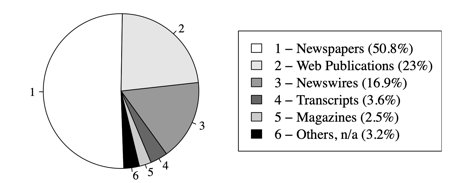
\includegraphics[width=4.2339in,height=1.6417in,width=\textwidth]{buerki-img002.png}
 
\end{styleStandard}

\begin{stylecaption}
Figure 2: Breakdown of document sources. Note: Newspapers include UK-wide titles as well as regional and local titles and free papers like the Metro. Web Publications include online portals of print media as well as online-only publications such as The Independent; Newswires include specialist Newswires such as Sport News or Global Banking News; Transcripts are of radio and TV programmes; Magazines include titles like The Spectator and the THES (100\% = 161,850 documents).
\end{stylecaption}

\begin{styleStandard}
Method
\end{styleStandard}

\begin{styleStandard}
The identification of relevant Brexit phraseology was carried out in three main steps. First, phraseological expressions were automatically extracted from each of the eight sub-corpora of 10 million words. Second, Brexit-related phraseological expressions were identified by contrasting expressions extracted from the Brexit sub-corpora with those extracted from non-Brexit sub-corpora. Finally, Brexit phraseology of the different phases of Brexit were compared with each other to find out to what extent these differed.
\end{styleStandard}

\begin{styleStandard}
To facilitate the first step, an operationalization of the concept of phraseological patterns as consecutive word sequences of two to seven words in length, occurring at least three times per million words in the corpus and forming a semantic unit was chosen (cf. also Buerki, 2020: ch. 3). This operationalises the earlier definition of phrases (= word sequences) that represent common ways (occurring {\textgreater}= 3/M) of putting things (semantic units) in a speech community. The particular speech community here are English speakers in the UK (co-referential with the discourse community whose discourses we seek to explore). 
\end{styleStandard}

\begin{styleStandard}
Measuring conventionality via frequency has definite drawbacks (as Wray, 2002:31, and others have pointed out, there are highly conventionalized phrases that are rare in general language use). However, it is felt that for present purposes, this drawback is sufficiently mitigated by the chosen low frequency threshold, which is very low compared to the range typically employed in corpus-linguistic research on formulaic language (e.g. 4/M in McCarthy and Carter, 2002:12; 10/M in Biber et al., 1999) and by not using frequency as the sole criterion. Further, although looking exclusively at consecutive word sequences biases the search towards the more fully lexically specific end of the phraseological spectrum, internal variable elements (e.g. \textit{a [nice/nasty/complete] surprise}) tend to follow a Zipfian distribution (Ellis 2012:35), meaning that the few most frequent of those elements account for most of the variation and can often be extracted \textit{in situ} if a low minimum frequency is chosen as is the case here. Nevertheless, it remains important when looking at results, to explore patterns around automatically identified sequences to establish a fuller picture of phraseological patterns. Finally, the idea that sequences should form semantic units (similar to the way single words or structurally complete phrases form semantic units) is an important additional constraint by which sequences are excluded that happen to be frequent purely because their constituent words are highly frequent (e.g. \textit{of the, and he}). Some sequences naturally only form semantic units once we allow for the implicit variable element (e.g. \textit{at the age of X}); these sequences were also deemed to possess semantic unity.
\end{styleStandard}

\begin{styleStandard}
  [Warning: Image ignored] % Unhandled or unsupported graphics:
%\includegraphics[width=4.7244in,height=3.8299in,width=\textwidth]{buerki-img003.emf}
 
\end{styleStandard}

\begin{stylecaption}
Figure 3: Summary of extraction procedure
\end{stylecaption}

\begin{styleStandard}
With this operationalization in place, a full, automatic extraction of operationalization-compliant sequences out of the eight sub-corpora was carried out. As mentioned above, a full automatic extraction has the advantage of allowing a maximally inter-subjective identification of relevant expressions as well as being able to deal with the large amounts of data available, whereas a manual identification of expressions would necessarily need to be highly selective with respect to the data that can be processed. The procedure described in Buerki (2016), summarized in Figure 3, was employed for the extraction of phraseological expressions. This procedure has previously achieved good accuracy (Buerki, 2016:23), a high recall due to a low frequency cut-off, and remains to date the only fully documented procedure that extracts consolidated word-sequences of different lengths, making it a tool well suited for present purposes. The eight lists so derived contained between 25,182 and 30,202 types of phraseological expressions. The number of word tokens contained in extracted expressions varied from 4.4 million words (4-Non-Brexit list) to 5.6 million words (5-Brexit list), out of the 10 million words contained in each of the eight sub-corpora.
\end{styleStandard}

\begin{styleStandard}
To identify Brexit-specific phraseology, the lists of expressions obtained from the four non-Brexit sub-corpora (1-Non-Brexit to 4-Non-Brexit in Figure 1) were first combined into a single master list of non-Brexit expressions containing all expression types from the four time periods (51,760 expression types in total). Second, each of the four lists derived from the Brexit sub-corpora (1-Brexit to 4-Brexit in Figure 1) were compared to the non-Brexit master list.
\end{styleStandard}

\begin{styleStandard}
As the goal was to identify Brexit-specific phraseology, the emphasis was, in the first instance, on phraseological patterns exclusive to the Brexit sub-corpora.\footnote{Some of the exclusive expressions do occur in the non-Brexit sub-corpora, but below the frequency at which they are here considered phraseological expressions.} Consequently, each of the four Brexit-sub-corpus derived lists were compared to the non-Brexit master list and any shared expressions were eliminated from the Brexit lists, leaving only expressions unique to the Brexit lists. Given the size of the corpora underlying the non-Brexit master list (four times 10 million words), it was felt that the risk of identifying an expression as Brexit phraseology in error because of a chance absence from the master list was low enough to be acceptable. For analysis, a Brexit expression master list was created, containing all expression types of the four periods, with frequencies across the periods summed. This list was ordered in decreasing order of frequency and the focus was on mid- to high frequency expressions across the periods.
\end{styleStandard}

\begin{styleStandard}
A secondary analysis was prepared of relative, rather than absolute Brexit expressions, that is, expressions that differ between Brexit and non-Brexit sub-corpora only in frequency (rather than in being present in one and absent in the other). For this purpose, expressions were identified that were far more frequent in the Brexit sub-corpora than in the non-Brexit sub-corpora by using the keyness formula suggested by Kilgarriff (2009), with a +N value of 100 added to each frequency count to prioritise mid- to high-frequency expressions (s. Kilgarriff, 2009). Consequently, an ordered list of absolute Brexit expressions, as well as one of relative Brexit expressions was created for analysis.
\end{styleStandard}

\begin{styleStandard}
Finally, to investigate the development of Brexit phraseology across the four periods of investigation, two further lists were prepared: a list of expressions exclusive to a single Brexit period, not found among the expressions of other periods, and a second list of expressions with frequencies that varied most across the four Brexit periods.\footnote{The top 8,000 Brexit expressions, together with their frequencies across all four periods, are searchable at \href{https://brexitphrases.herokuapp.com/}{\textstyleInternetlink{brexitphrases.herokuapp.com}}.}
\end{styleStandard}

\begin{styleStandard}
As the number of expressions on each of these lists was far too large for individual analysis, the lists were ordered according to likely typicality for each list’s focus, providing a rigorous and maximally inter-subjective basis for a judged selection and analysis of individual expressions and groups of expressions. The results of these selections and their analyses are presented in the next section; their implications are discussed in the final section of this chapter.
\end{styleStandard}

\begin{listWWNumxxiileveli}
\item 
\begin{stylelsSectioni}
Results
\end{stylelsSectioni}
\end{listWWNumxxiileveli}
\begin{styleStandard}
This section presents results that allow us to draw conclusions regarding the questions set out above. We start by considering the data on the question of whether the Brexit discourse is more phraseologically rich than comparable discourses, that is, whether it has a higher density of phraseological expressions – something that, while not previously formally analysed, may be suggested by popular comments about the discourse being reduced to slogans or by the finding that there is a large amount of metaphor applied to the Brexit discourse, much of it via set expressions and phrases (cf. Charteris-Black, 2019:2). Table 2 shows the proportion of word tokens that are part of automatically extracted phraseological expressions in Brexit and non-Brexit texts across the four periods of study. Non-Brexit texts consistently show a notably lower density of phraseological expressions.
\end{styleStandard}

\begin{flushleft}
\tablefirsthead{}
\tablehead{}
\tabletail{}
\tablelasttail{}
\begin{supertabular}{m{1.5462599in}m{1.5462599in}m{1.5462599in}}
 &
\centering Brexit texts &
\centering\arraybslash non-Brexit texts\\\hline
Period 1 &
\centering 0.63 &
\centering\arraybslash 0.46\\
Period 2 &
\centering 0.53 &
\centering\arraybslash 0.46\\
Period 3 &
\centering 0.49 &
\centering\arraybslash 0.44\\
Period 4 &
\centering 0.56 &
\centering\arraybslash 0.46\\
mean &
\centering 0.55 &
\centering\arraybslash 0.46\\
\end{supertabular}
\end{flushleft}
\begin{stylecaption}
Table 2: Phraseological density of Brexit and non-Brexit texts. Note: figures represent the ratio proportion of total word tokens that are part of phraseological expressions. For key to periods, see Table 1.
\end{stylecaption}

\begin{styleStandard}
Before we can conclude, however, that Brexit discourse is more phraseologically dense, it is worth considering whether the difference in density might be influenced by the difference between a topically more uniform set of texts (Brexit texts all contain the word \textit{Brexit} and might therefore be in a sense \textit{about} Brexit) and a topically diverse set of texts (non-Brexit texts cover all other topics). If topical diversity might be linked to a greater diversity of phraseological expression, it could mean that it is more difficult to identify conventional turns of phrase in topically diverse texts (leading to fewer expressions being identified) because there is less repetition of the same phraseological patterns. It seems, however, that although there may well be topic-related influences, the conclusion of clearly higher phraseological density in Brexit texts is justified: first, although Brexit texts are at least partially about Brexit because they contain the word \textit{Brexit}, the phenomenon of Brexit is characteristically one that touches all areas of life. That is to say, there may well be discussion of Brexit in texts about sport, cooking or money matters as well as politics and news, whereas similarly, non-Brexit texts may cover any of these topics. In this sense, Brexit texts still contain remarkable topical diversity. Second, to see if indeed non-Brexit phraseology was more diverse, two indicators show no clear support for notably more diversity in non-Brexit phraseology: in terms of type-token ratios of expressions, Brexit texts show an average type to token ratio of 1:66 among phraseological expressions, for non-Brexit texts of 1:70, indicating only a somewhat elevated diversity in expressions rather than a dramatic difference. In terms of how internally diverse Brexit expressions and non-Brexit expressions are, one might look at what proportion of expression types and tokens are shared between pairs of periods across Brexit and non-Brexit texts: out of a mean of 30,539 expression types identified per period in Brexit texts (range: 28,040 – 34,188), on average 47.9\% are shared with each of the other three periods. In the case of non-Brexit texts, the figure is notably higher at 57.5\% (mean of types 25,693; range 25,182 – 26,600), indicating less diversity within the phraseology of non-Brexit texts, rather than more diversity. For expression tokens, the equivalent figures are 63\% for Brexit texts and 71\% for non-Brexit texts. The comparatively elevated phraseological density of Brexit texts therefore seems to be a genuine feature of the Brexit discourse rather than attributable to differences in topical diversity.
\end{styleStandard}

\begin{styleStandard}
Turning now to examples of Brexit expressions, it is clear that these are multi-faceted and rich. They range from multi-word terms to slogans to collocations and other usual sequences, many of which are embedded in new phraseological patterns that have become conventional ways of talking about Brexit-related issues. Some of the expressions are new coinages, some are used in new senses or previously existed only in specialist discourses. We start by looking at multi-word terms. Among the large number of multi-word terms are examples (1) to (17).\footnote{Square brackets, [], indicate optional variable elements of an expression, a slash indicates alternatives.}
\end{styleStandard}


\setcounter{listWWNumxxivleveli}{0}
\begin{listWWNumxxivleveli}
\item 
\begin{styleListParagraph}
the single market and customs union
\end{styleListParagraph}
\item 
\begin{styleListParagraph}
[allow/end] free movement / freedom of movement
\end{styleListParagraph}
\item 
\begin{styleListParagraph}
[trigger] article 50
\end{styleListParagraph}
\item 
\begin{styleListParagraph}
[avoid/return to] a hard [Irish] border
\end{styleListParagraph}
\item 
\begin{styleListParagraph}
[cut/reduce] net migration
\end{styleListParagraph}
\item 
\begin{styleListParagraph}
a second referendum
\end{styleListParagraph}
\item 
\begin{styleListParagraph}
the cliff edge
\end{styleListParagraph}
\item 
\begin{styleListParagraph}
a Brexit deal
\end{styleListParagraph}
\item 
\begin{styleListParagraph}
the remain / leave camp
\end{styleListParagraph}
\item 
\begin{styleListParagraph}
hard Brexiteers
\end{styleListParagraph}
\item 
\begin{styleListParagraph}
hard / soft Brexit
\end{styleListParagraph}
\item 
\begin{styleListParagraph}
the will of the [British] people
\end{styleListParagraph}
\item 
\begin{styleListParagraph}
project fear
\end{styleListParagraph}
\item 
\begin{styleListParagraph}
the British people
\end{styleListParagraph}
\item 
\begin{styleListParagraph}
red line[s]
\end{styleListParagraph}
\item 
\begin{styleListParagraph}
personal attack[s]
\end{styleListParagraph}
\item 
\begin{styleListParagraph}
Brexit uncertainty
\end{styleListParagraph}
\end{listWWNumxxivleveli}
\begin{styleStandard}
These have become well-established and widely used across the different phases of Brexit. (1) to (3) are technical terms that have been catapulted into widespread use in the Brexit discourse. One remarkable feature is how, around these expressions, extended phraseological patterns and very clear collocational preferences have arisen that are evidently the product of rapid conventionalization: for example, frequent patterns involving either the whole phrase in (1), or one of the co-ordinated expressions, include \textit{[in/outside/access to/stay in/remain in/leave] the [European/EU’s/EU] single market. }Similarly, (2), (3), (4) and (5) have their preferred verbal collocates as indicated. Expressions that are topically similar to (4) include \textit{the Irish border issue }and \textit{the Good Friday Agreement, }the latter an example of a relative Brexit expression (occurring in non-Brexit texts, but at a much lower frequency). This cluster highlights the magnitude of difficulties created by Brexit on the island of Ireland. Perhaps the most interesting case of collocational preference is (3) which has developed a virtually exclusive preference for forms of the verb \textit{to trigger}. The alternative\textit{ invoke article 50} makes a brief appearance in phase two of Brexit, but is unable to establish itself. The metaphorical triggering seems to suggest the setting in motion of an unstoppable train of events (whereas a revocation can follow an invocation), forcing a particular conceptualisation of events. There are other examples where there seems to be a competition between alternative phrasings, with the existence of a dominant pattern that is (or becomes) the conventional way of expression: (6) is by far the most usual way of referring to the idea of another referendum on the UK’s membership of the EU to be held after the Brexit referendum of 2016. However, in period 4, there are other expressions for the same concept (\textit{a people’s vote}; \textit{a confirmatory referendum};\textit{ a final say referendum}), none of which reach the frequency of \textit{a second referendum}. This appears to show that once a phraseological expression is established as the usual way to express a meaning, it is very difficult to challenge it, even if the conventional expression arguably carries with it a certain (possibly undesirable) conceptualisation of the world: the alternatives to \textit{a second referendum} seek to avoid the implication of a re-run of the 2016 referendum, for example. Similarly, (7) is a conventional expression for referring to a sudden, disorderly exit from the EU,\footnote{\textit{disorderly exit }itself only just makes the cut for being a phraseological expression in its own right in period 4, but in no other period.} but arguably carries with it the vivid picture of catastrophe that many Brexit-supporting language users might wish to dispel. Similar, arguably forced, conceptualisations built into phraseological expressions are evident in (8) reflecting the language of deal-making (cf. Achilleos-Sarll and Martill, 2019)\footnote{The more neutral \textit{withdrawal agreement} only becomes a phraseological expression in period 4.}, as well as in (9) to (13). (14) to (17) are expressions that shine a light on concepts evidently prominent in the discourse – the concept of a nation, of tough negotiation stances, the bruising arguments, and of the effects of Brexit. A shift in convention is observable in the data in relation to labels applied to people supporting or opposing Brexit: \textit{the remain camp} and \textit{the leave camp} (notably militaristic expressions, cf. Achilleos-Sarll and Martill, 2019) have fallen out of use as phraseological expressions by period 4, being replaced by snappier single word expressions (e.g. \textit{remainers / leavers}, also (10) and similar). \textit{leavers and remainers}, as per (18), is a binomial attested with increasing frequency from period 2 onwards, but there are also attestations of the form \textit{remainers and leavers} in the data, showing that this expression has not yet reached the status of \textit{irreversible }binomial. A similar observation holds for (1), which is far more frequent in the cited form, but also appears as \textit{the customs union and [the] single market} and so has not solidified to an irreversible binomial either, showing that these expressions are still in the process of being fully established.
\end{styleStandard}

\begin{listWWNumxxivleveli}
\item 
\begin{styleListParagraph}
leavers and remainers
\end{styleListParagraph}
\item 
\begin{styleListParagraph}
our children and grandchildren (periods 1\&3)
\end{styleListParagraph}
\item 
\begin{styleListParagraph}
parents and grandparents (period 1)
\end{styleListParagraph}
\item 
\begin{styleListParagraph}
strong and stable (periods 3\&4)
\end{styleListParagraph}
\item 
\begin{styleListParagraph}
our [European] friends and partners (period 4)
\end{styleListParagraph}
\end{listWWNumxxivleveli}
\begin{styleStandard}
The binomials shown in (19) to (22) are more clearly irreversible in their order. Particularly fascinating are (19) and (20) – not only are they relative Brexit expressions (they occur at low frequency in non-Brexit texts and predate the period of observation as phraseological expressions), they are also specific to period 1, the pre-referendum period. (19) speaks to the epochal gravity and enormity of the Brexit decision (demonstrated by typical usages such as ‘with our children and grandchildren 's future at stake […]’) and to an extent, they both also stand for the two sides of the argument: a proportion of contexts for (19) suggests that ‘our children and grandchildren’ would wish to remain, whereas the referents of (20) tend in most contexts to be thought of as natural leavers (e.g. ‘Cameron has pleaded with parents and grandparents to vote to stay’).
\end{styleStandard}

\begin{styleStandard}
There are, however, irreversible binomials that were formed within the Brexit discourse itself: (21) and (22) are examples of (deliberate) coinages that are also closely tied to specific periods of Brexit: (21) appears in period 3 and peaks in period 4 (the run-up to the June 2017 general election), and (22) is exclusive to period 4 where it serves as a label for the EU. Whereas (62) and (69), below, conceptualise the EU as (ex-) family (cf. also Islentyeva, 2019), (22) appears friendlier, but with the sting of a far more clearly distanced relationship. The nature of (22) as a deliberate coining that appears in official communications and pronouncements in period 4, opens the possibility that the distancing might be another example of attempted forced conceptualisation.
\end{styleStandard}

\begin{styleStandard}
Further, the category of phrasal verbs and other verbal patterns is exemplified by expressions (23) to (32).\footnote{In these examples as elsewhere, \textit{X} stands for a non-optional variable element.}
\end{styleStandard}

\begin{listWWNumxxivleveli}
\item 
\begin{styleListParagraph}
pressed on X
\end{styleListParagraph}
\item 
\begin{styleListParagraph}
lashed out at X
\end{styleListParagraph}
\item 
\begin{styleListParagraph}
press ahead with X
\end{styleListParagraph}
\item 
\begin{styleListParagraph}
argued for X
\end{styleListParagraph}
\item 
\begin{styleListParagraph}
free up [money/£350 million a week/cash/…]
\end{styleListParagraph}
\item 
\begin{styleListParagraph}
leave on WTO terms
\end{styleListParagraph}
\item 
\begin{styleListParagraph}
revised down
\end{styleListParagraph}
\item 
\begin{styleListParagraph}
[slumped/fell/tumbled] by as much as X
\end{styleListParagraph}
\item 
\begin{styleListParagraph}
raised the prospect of X
\end{styleListParagraph}
\item 
\begin{styleListParagraph}
have a negative impact on X
\end{styleListParagraph}
\end{listWWNumxxivleveli}
\begin{styleStandard}
Expressions (23), as in ‘Mr Barclay was pressed on what would happen if …’, to (26) by virtue of appearing (at above-threshold frequency) exclusively in Brexit-related texts appear to reveal something of the way in which social actors behave in public discourse: they might be evasive (23), brash in tone (24), stubborn (25), and engaged in permanent arguments (26), in addition to indulging in \textit{personal attacks }(16). (27) is found in contexts where it is argued that leaving the EU will result in improved state finances, (28) could be seen as an alternative rendering of the situation referred to in (7) as \textit{the cliff edge }and (29) to (32) chime with (17) above in indicating recurrent patterns related to the impact of Brexit. 
\end{styleStandard}

\begin{styleStandard}
A further category of expression are slogans, where deliberate coinages are most clearly in evidence. It is noteworthy that such slogans show up in the data (which after all do not include political speeches as such, nor parliamentary proceedings) – it seems the originators of these expressions are influential enough to be able to achieve wide dissemination. These expressions show a tendency to simplify issues and are ideologically highly charged. (12), (13), (21) and (22), discussed earlier, share with these expressions their likely or certain status of being deliberate coinages.
\end{styleStandard}

\begin{listWWNumxxivleveli}
\item 
\begin{styleListParagraph}
the best possible deal
\end{styleListParagraph}
\item 
\begin{styleListParagraph}
Brexit means Brexit
\end{styleListParagraph}
\item 
\begin{styleListParagraph}
no deal is better than a bad deal
\end{styleListParagraph}
\item 
\begin{styleListParagraph}
take back control [of [immigration / our laws, borders, money and trade / ...]]
\end{styleListParagraph}
\item 
\begin{styleListParagraph}
the best deal [for [families and businesses / Britain / every part of the UK / ...]]
\end{styleListParagraph}
\end{listWWNumxxivleveli}
\begin{styleStandard}
Examples of other usual sequences and phraseological patterns are shown in (38) to (52) and include epoch references as in (38) to (40); the latter is a relative Brexit expression (occurring at far lower frequencies in non-Brexit texts) and suggests that Brexit is being perceived as an event of a magnitude that invites comparison to World War II. Various patterns referencing uncertainty (including the difficulty of predictions as in (42)) and repercussions of Brexit, (41) to (50), are also evident. Further clues to the societal climate (51) and the seemingly ever-present possibility of short-term dramatic shifts in situations (52), are also apparent.
\end{styleStandard}

\begin{listWWNumxxivleveli}
\item 
\begin{styleListParagraph}
since the referendum / since the Brexit vote / following Brexit
\end{styleListParagraph}
\item 
\begin{styleListParagraph}
in the post-Brexit [era/world] / [in] post-Brexit Britain
\end{styleListParagraph}
\item 
\begin{styleListParagraph}
since the Second World War
\end{styleListParagraph}
\item 
\begin{styleListParagraph}
fall in the value of the pound / the weak[er] pound
\end{styleListParagraph}
\item 
\begin{styleListParagraph}
[weaker/lower/less/better/more/stronger] than expected
\end{styleListParagraph}
\item 
\begin{styleListParagraph}
the uncertainty surrounding [Brexit/the status of EU nationals/the UK's future relationship with the EU/...]
\end{styleListParagraph}
\item 
\begin{styleListParagraph}
because of Brexit / as a result of [Brexit/leaving [the EU]]
\end{styleListParagraph}
\item 
\begin{styleListParagraph}
what Brexit will mean for X
\end{styleListParagraph}
\item 
\begin{styleListParagraph}
[concerned about] the impact/effect of Brexit [on X]
\end{styleListParagraph}
\item 
\begin{styleListParagraph}
the potential impact of X
\end{styleListParagraph}
\item 
\begin{styleListParagraph}
X [has] warned [of] Y / warning that [Brexit could] X
\end{styleListParagraph}
\item 
\begin{styleListParagraph}
[what] Brexit means [for [business/Wales/the future of X/...]]
\end{styleListParagraph}
\item 
\begin{styleListParagraph}
the [pressing/critical/biggest/major/real/…] issues facing X
\end{styleListParagraph}
\item 
\begin{styleListParagraph}
the anger [of X / at X / among X / …]
\end{styleListParagraph}
\item 
\begin{styleListParagraph}
at the time of writing
\end{styleListParagraph}
\end{listWWNumxxivleveli}
\begin{styleStandard}
The final category, proverbs and idioms, is exemplified in (53) to (55). Their comparatively high frequency in the discourse is highly notable because pure idioms and proverbs are rare in normal language use (Moon, 1998). (53) is an allusion to the proverb \textit{You can’t have your cake and eat it} and occurs in texts in relation to aspects of the Brexit negotiating position of the UK government, as noted in previous analyses (Charteris-Black, 2019; Musolff, 2019). In this sense, it could be seen as challenging the assertive \textit{red line[s]} (15) in the negotiations that refer to positions that will be preserved under all circumstances. (54) is similarly used as a criticism of negotiating positions taken by the UK government, and finds its counterpoint perhaps in the accusation of (75). (55) is an expression specific to period 4; contexts suggest it is an evaluation of the series of exit date extensions of that period. 
\end{styleStandard}

\begin{listWWNumxxivleveli}
\item 
\begin{styleListParagraph}
[have] cake and eat[ing] it
\end{styleListParagraph}
\item 
\begin{styleListParagraph}
cherry pick[ing]
\end{styleListParagraph}
\item 
\begin{styleListParagraph}
kick[ing] the can down the road (period 4)
\end{styleListParagraph}
\end{listWWNumxxivleveli}
\begin{styleStandard}
Before concluding the review of examples of Brexit phraseology, it is important to highlight examples of discontinuity in the phraseology of Brexit across the four time periods covered. Above, we reviewed figures showing that, on average, each period shares 47.9\% of its Brexit expression types and 63\% of expression tokens with each of the other periods. Clearly, there is therefore continuity in Brexit expressions across various periods and most expressions so far reviewed occur in most periods.\footnote{It is likely also that many of these expressions will remain part of the language for the long term – (39), for example, might well become a staple phrase similar to (40).} But there are also significant shifts: we have already encountered shifts in designations of supporters and detractors of Brexit from (9) to (18). Similarly, examples (56) to (75), which occur above the phraseological threshold (3/M) in only one or two periods, show that there is a clear sense in which different periods have their own phraseology.
\end{styleStandard}

\begin{listWWNumxxivleveli}
\item 
\begin{styleListParagraph}
referendum on Britain’s membership of the EU (period 1)
\end{styleListParagraph}
\item 
\begin{styleListParagraph}
a European army (period 1)
\end{styleListParagraph}
\item 
\begin{styleListParagraph}
economic migrants (period 1)
\end{styleListParagraph}
\item 
\begin{styleListParagraph}
ever closer union (period 1)
\end{styleListParagraph}
\item 
\begin{styleListParagraph}
concerns about immigration (period 1)
\end{styleListParagraph}
\item 
\begin{styleListParagraph}
invoke article 50 (period 2)
\end{styleListParagraph}
\item 
\begin{styleListParagraph}
divorce proceedings (period 2)
\end{styleListParagraph}
\item 
\begin{styleListParagraph}
in the aftermath of the Brexit vote (period 2)
\end{styleListParagraph}
\item 
\begin{styleListParagraph}
the fallout from the Brexit vote (period 2)
\end{styleListParagraph}
\item 
\begin{styleListParagraph}
regulatory divergence (period 3)
\end{styleListParagraph}
\item 
\begin{styleListParagraph}
speech in Florence (period 3)
\end{styleListParagraph}
\item 
\begin{styleListParagraph}
[a/the][second] meaningful vote (period 3)
\end{styleListParagraph}
\item 
\begin{styleListParagraph}
a constitutional crisis (periods 3 and 4)
\end{styleListParagraph}
\item 
\begin{styleListParagraph}
[Brexit] divorce bill (periods 3 and 4)
\end{styleListParagraph}
\item 
\begin{styleListParagraph}
fourth meaningful vote (period 4)
\end{styleListParagraph}
\item 
\begin{styleListParagraph}
the Benn act (period 4)
\end{styleListParagraph}
\item 
\begin{styleListParagraph}
reaching an agreement is still possible (period 4)
\end{styleListParagraph}
\item 
\begin{styleListParagraph}
more and more difficult (period 4)
\end{styleListParagraph}
\item 
\begin{styleListParagraph}
proroguing parliament (period 4)
\end{styleListParagraph}
\item 
\begin{styleListParagraph}
abject surrender (period 4)
\end{styleListParagraph}
\item 
\begin{styleListParagraph}
if Britain leaves the EU (absent in period 2)
\end{styleListParagraph}
\item 
\begin{styleListParagraph}
recognition that X (absent in period 4)
\end{styleListParagraph}
\end{listWWNumxxivleveli}
\begin{styleStandard}
In some cases, period-specific phraseological expressions have been replaced by other expressions in subsequent periods – (56) was replaced by \textit{the referendum }or \textit{the Brexit referendum}, likely for reasons of economy of expression. (57) to (60), as well as (19) and (20) as noted earlier, appear to express concerns largely of the pre-referendum period. (63) and (64) are among expressions reflecting the shock of the immediate post-referendum period and the processes that had to be initiated, e.g. (61) and (62). Periods 3 and 4 seem to have some overlap in their concerns and expressions of these periods document wranglings over agreements between the EU and the UK, or over the lack of agreements, as in (65), (68) to (75).
\end{styleStandard}

\begin{styleStandard}
Other expressions appear (and disappear) with the relevance of their denotations: \textit{meaningful vote }in (67) and (70) – a technical term for a vote in parliament (repeated several times) on the withdrawal agreement negotiated by former Prime Minister May – became irrelevant shortly after the events, similarly (66).
\end{styleStandard}

\begin{styleStandard}
By contrast to expressions that only appear in one or two periods, (76) and (77) are examples of expressions that are (conspicuously) absent from only one of the Brexit periods. (77), for example, appears in contexts where social actors concede a point with an amount of humility – its fall from a top frequency of over 7/M in period 1 to disappearance from the discourse in period 4 may be a further indicator of polarisation and a worsening of the tone of the discourse.
\end{styleStandard}

\begin{styleStandard}
There are also notable shifts in frequencies of expressions that appear across periods: (6), for example, while frequent in all four periods, shows a generally increasing frequency development, whereas mentions of (5) follow a generally decreasing trend. Former Prime Minister May’s slogan in (35) comes in at over 8 times per million words in period 2, but its frequency has halved by period 4 while her slogan in (34), similarly, is very frequent in periods 2 and 3, but halves in frequency for period 4.
\end{styleStandard}

\begin{styleStandard}
The appearance and disappearance of expressions in specific periods shows that where needed, conventionalised expressions can be brought into use in a speech community over very short intervals, indeed. This seems clear evidence for the existence of pro-tem phraseological expressions (to borrow Seidlhofer’s term), not just at the micro-level of small group communication (cf. Seidlhofer, 2009), but at the level of a complete speech community such as the speakers of British English. From the point of view of phraseological theory, it is stunning to see widely used and circulated pro-tem phraseology documented in the data – as well as seeing such a rapid creation of new phraseological expressions and to observe expressions as they are formed, such as the binomials that are not fully irreversible. Both in terms of the significance of pro-tem phraseological expressions at the level of a speech community as well as the rapidity of phraseological development, these observations open up areas of phraseological study that require more investigation and reflection, but they are in agreement with recent findings on the rapidity of phraseological change (cf. Buerki, 2019).
\end{styleStandard}

\begin{styleStandard}
Having quantified aspects of the phraseology of Brexit and reviewed examples showing the richness and diversity as well as the continuity and discontinuity of Brexit phraseology, we are now in a position to discuss, in the final section, answers to the questions posed at the outset.
\end{styleStandard}


\setcounter{listWWNumxxiileveli}{0}
\begin{listWWNumxxiileveli}
\item 
\begin{stylelsSectioni}
Discussion
\end{stylelsSectioni}
\end{listWWNumxxiileveli}
\begin{styleStandard}
Results presented in the preceding section now allow us to attempt a reading of the discourses of Brexit through their phraseology. Three areas seem worth particular mention:
\end{styleStandard}

\begin{styleStandard}
First, the domains and meanings encoded phraseologically, in other words, those meanings sufficiently frequently communicated to develop usual turns of phrase used in the Brexit discourse, allow us to read some of the concerns of the Brexit discourse, what is happening within society and what the issues of public concern are. At a necessarily general level, these include: 
\end{styleStandard}

\begin{listWWNumxxxvleveli}
\item 
\begin{styleListParagraph}
An impression of the complexity of Brexit (the specialist multi-word terms that have entered common use in the discourse)
\end{styleListParagraph}
\item 
\begin{styleListParagraph}
Conversely, efforts to present Brexit in simplistic terms, cf. the slogans in (33) to (37)
\end{styleListParagraph}
\item 
\begin{styleListParagraph}
Indicators of the roughness of much of the discourse: (16), (17), (23) to (26), (77)
\end{styleListParagraph}
\item 
\begin{styleListParagraph}
Topical preoccupations on borders and immigration, e.g. (4), (5), (36), (58) to (60), cf. also Mair (2019)
\end{styleListParagraph}
\item 
\begin{styleListParagraph}
Polarisation, with many terms appearing in opposing sets, cf. further discussion below
\end{styleListParagraph}
\item 
\begin{styleListParagraph}
A very deep sense of uncertainty, expressed in (17), (29) to (32), (41) to (52), (63), (64)
\end{styleListParagraph}
\item 
\begin{styleListParagraph}
The epoch-defining status of Brexit as in (38) to (40)
\end{styleListParagraph}
\item 
\begin{styleListParagraph}
A realization of deepening crisis within the discourse itself with the emergence of (68), perhaps emblematically (73) and the collocation (74) brought back from the obscurity of history.
\end{styleListParagraph}
\end{listWWNumxxxvleveli}
\begin{styleStandard}
The data here show that popularly recognised high-profile expressions, e.g. (10) or (11), do reflect the phraseology of Brexit, but there are many more subtle patterns that have slipped under the radar while just as much part of Brexit phraseology. The bottom-up, comprehensive procedure employed in this study was able to bring these to the surface as well. Some of them are less noticed patterns that are able to add extra insight that is important: the patterns around uncertainty and consequences of Brexit, for example, are more extensive and prominent than perhaps generally acknowledged and verbal patterns revealing aspects of the tone of the discourse are equally highly revealing.
\end{styleStandard}

\begin{styleStandard}
Second, diachronic aspects of the analysis suggest that the discourse itself is fast-paced and ever changing. On the one hand, this can be read as speaking to the ever new challenges and consequences of Brexit emerging and requiring discussion (e.g. in (4) and (6)), and thus further to the sense of instability and insecurity evident within the discourse. There appear to be expressions that are tied to particular phases of Brexit in a way that makes them appear dated or out of place in other periods. In this respect, there are phraseologies (plural) of Brexit, as well as a common phraseological bedrock of Brexit expressions. This points similarly to a plurality of discourses within the overall Brexit discourse.
\end{styleStandard}

\begin{styleStandard}
On the other hand, variation and fast change also reveal intense conflicts over alternative conceptualisations of key aspects of the Brexit narrative that are played out to a notable extent in phraseology: opposing expressions, some deliberately coined, some more naturally occurring, are vying for the status of the usual way in which their meaning is expressed (and with it the usual way in which that domain is conceptualized). Cases in point are the expressions (28) vs. (7) as well as (15)\textit{ }vs. (54) and (53) vs. (75)\textit{. }These are by the end of the period of observation still very much contested. As observed, no one side or tendency has been successful in getting all ‘their’ conceptualisations accepted in the community – there remains a diversity of ideologically incompatible conceptualisations in current use, pointing to an ongoing and vast array of domains that remain contested in the discourse. There are some aspects that have been settled –\textit{ people’s vote} vs. \textit{second referendum,} are shown to have been settled in favour of the second conceptualisation, for example, but these are relatively few. Notably, (76), \textit{if Britain leaves the EU}, shows a high frequency in the pre-referendum period, but disappears as a common turn of phrase in period 2 (the immediate post-referendum period) indicating that the most fundamental question (whether or not Brexit will happen) appears settled. However, the data show that it re-emerges as a common turn of phrase in periods 3 and 4, showing that by the end of the period of observation, the most fundamental question regresses into the category of what is contested within society.
\end{styleStandard}

\begin{styleStandard}
Third, beyond struggles in the diachronic development of phraseological expressions, Brexit phraseology in general very often seems ideologically charged, as shown in examples (7), (8), (13), (27), (28) and (33) to (37), in particular. This indicates the limited possibility of neutrality in this discourse: participants in the discourse cannot but take sides in one way or another if they wish to speak. Particularly in cases where expressions force a certain conceptualisation of events, often through conceptual metaphors (Lakoff and Johnson, 1980), deliberate coinages feature strongly. This attempted forced conceptualisation of a domain, particulary in political discourse, is sometimes labelled ‘framing’ (Lakoff, 2010) and has been extensively documented by Lakoff. The finding of a concentration of attempted forced conceptualisation in phraseological expressions indicates that phraseology itself appears to be instrumentalised (not to say \textit{weaponised}) by actors in the discourse.\footnote{Wintour (2020) reports that ‘Foreign Office staff have been banned from using certain words and phrases in discussing Brexit – including “implementation period”, “no deal”, “special partnership” and even Brexit itself […]’} However, slogans and other deliberate coinages are joined by more naturally conventionalised expressions and many of the coined terms are themselves embedded in usual phrasings, while other attempted coinages are very short-lived or so evidently counter-factual that they can now only be used with irony as is the case with (21) and so these linguistic power struggles are not artificial in nature. Rather, they can reasonably be read to reflect societal struggles, some of which have recently been labelled \textit{culture wars} (Sobolewska and Ford, 2020).
\end{styleStandard}

\begin{styleStandard}
A notable additional feature uncovered is that the Brexit discourse is more peppered with phraseology than comparable discourses, perhaps reflecting an entrenchment of often polarized views among those participating in the discourse. Likely parallels can also be drawn to what Szerszunowicz (2015) termed a \textit{periodic growth of phrasemes}, an intensive increase in the number of phraseological expressions ‘triggered by an important event in the history of a particular culture’ (2015:103). Szerszunowicz demonstrates the phenomenon using the 1989 change of system in Poland which ‘influenced greatly all spheres of life in Poland, such as politics, economy, culture’ (2015:103) and led to the creation of a great number of new phraseological expressions. Although Szerszunowicz primarily documents an increase in types (rather than specifically an increase in the phraseological density of texts, i.e. of tokens), she notes a general colloquialisation of public discourse which included an increased use of idioms and sayings as well as that ‘the ability to include many [scientific] terms [and expressions] into public speeches was an important element’ (2015:108). The observation that the Brexit discourse is more phraseologically dense than discourses on other topics (as well as the parallels regarding the creation of many new expression types) could therefore also point to the magnitude of change (in this case in all spheres of life in Britain) brought on by Brexit – a finding that contributes intriguing facets of insight to the emerging field of Brexit studies.
\end{styleStandard}

\begin{styleStandard}
To conclude, I would like to propose three theses, based on discussed findings. These should serve to move the current state of research forward, firstly by underpinning and supporting findings of existing work that has sought to bring phraseology to bear on discourse analytical questions. Secondly by making it more attractive to overtly declare phraseological work in discourse analysis as such and in so doing benefit from the support of phraseological theory, and finally by encouraging the use of phraseological means of reading discourses to a far fuller extent in the interest of further advances in discourse analysis and in the interest of the stretching, testing and mapping out of the boundaries of the validity of these theses:
\end{styleStandard}


\setcounter{listWWNumxxxivleveli}{0}
\begin{listWWNumxxxivleveli}
\item 
\begin{styleListParagraph}
Phraseological patterns allow deep insight into what is happening within society, what the issues of public concern are, what is contested or settled (including how this changes over time) – in short, they allow us to read the discourses of a community. The likely precondition to this is a robust, data-led identification of relevant patterns. This first thesis is, so the hope, borne out by the results presented, but also leads to the realisation of thesis 2.
\end{styleListParagraph}
\item 
\begin{styleListParagraph}
Discourses crystallise (to a remarkable extent) in phraseology. This is regardless of whether the items of phraseology under scrutiny are attempts at deliberate coinages (where successful, these develop their own embeddings and extended patterns through natural conventionalisation) or not and whether they are pro-tem items or patterns that are part of the language over longer periods of time. Indeed, where diachronic aspects can be assessed, this necessarily adds important additional angles (cf. Mair, 2019) even over short periods of time, such as the 44-month period investigated in this study.
\end{styleListParagraph}
\item 
\begin{styleListParagraph}
Phraseological theory explains why all this should be the case: 1 and 2 above are not merely empirical curiosities but follow from the essence of phraseology as common turns of phrase that represent conventional, usual ways of putting things in a speech community. As such, items of phraseology that are the result of communal discursive practice and negotiation (part of the sediment of social practice, to speak with Bourdieu, 1977), are by virtue of their nature salient and contain not only more propositional meaning than other items of language but carry pre-understandings and conceptualisations of reality (Feilke, 1994, Lakoff, 2010). That is why they allow deeply penetrating access to the discourses of a community.
\end{styleListParagraph}
\end{listWWNumxxxivleveli}

\setcounter{listWWNumxxiileveli}{0}
\begin{listWWNumxxiileveli}
\item 
\begin{stylelsSectioni}
References
\end{stylelsSectioni}
\end{listWWNumxxiileveli}
\begin{styleStandard}
Achilleos-Sarll, C., \& Martill, B. (2019). Toxic Masculinity: Militarism, Deal-Making and the Performance of Brexit. In\textit{ Gender and Queer Perspectives on Brexit}. Cham: Palgrave Macmillan. pp. 15-44.
\end{styleStandard}

\begin{styleStandard}
Allerton, D. J. (1984). Three (or four) levels of word cooccurrence restriction. \textit{Lingua,} 63(1):17–40.
\end{styleStandard}

\begin{styleStandard}
Biber, D., Johansson, S., Leech, G., Conrad, S., and Finegan, E. (1999).\textit{ Longman grammar of spoken and written English. }Harlow: Pearson Education.
\end{styleStandard}

\begin{styleStandard}
Biber, D. (2006). Stance in spoken and written university registers. \textit{Journal of English for Academic Purposes}, 5(2):97–116.
\end{styleStandard}

\begin{styleStandard}
Bourdieu, P. (1977).\textit{ Outline of a theory of practice}. Cambridge: Cambridge University Press.
\end{styleStandard}

\begin{styleStandard}
Buckledee, Steve. 2018.\textit{ The Language of Brexit: How Britain Talked Its Way Out of the European Union}. London: Bloomsbury.
\end{styleStandard}

\begin{styleStandard}
Buerki, A. (2014).\textit{ N-gram processor 0.4.} [computer software]. (\url{http://buerki.github.io/ngramprocessor/}) (Accessed 13/11/2014).
\end{styleStandard}

\begin{styleStandard}
Buerki, A. (2016).\textit{ }Formulaic sequences: a drop in the ocean of constructions or something more significant?\textit{ European Journal of English Studies}, 20(1):15–34.
\end{styleStandard}

\begin{styleStandard}
Buerki, A. (2017). Frequency consolidation among word n-grams : A practical procedure. In Mitkov, R. (ed), \textit{Computational and Corpus-based Phraseology, Lectures in Computer Science}. Cham: Springer. pp. 432–446.
\end{styleStandard}

\begin{styleStandard}
Buerki, A. (2019). Furiously Fast. On the speed of change in Formulaic Language. \textit{Yearbook of Phraseology,} 10.\textit{ }pp. 5-38
\end{styleStandard}

\begin{styleStandard}
Buerki, A. (2020).\textit{ Formulaic Language and Linguistic Change. }Cambridge: Cambridge University Press.
\end{styleStandard}

\begin{styleStandard}
Burger, H., Häcki Buhofer, A., and Sialm, A. (1982\textit{). Handbuch der Phraseologie. }Berlin: de Gruyter.
\end{styleStandard}

\begin{styleStandard}
Burger, H., Dobrovol’skij, D., Kühn, P., and Norrick, N. R. (2007). Phraseology: Subject area, terminology and research topics. In Burger, H., Dobrovol’skij, D., Kühn, P., and Norrick, N. R. (eds),\textit{ Phraseology: an international handbook of contemporary research. }Berlin: de Gruyter. 11-19.
\end{styleStandard}

\begin{styleStandard}
Bybee, J. L. (2010).\textit{ Language, usage and cognition.} Cambridge: Cambridge University Press.
\end{styleStandard}

\begin{styleStandard}
Celli, F., Stepanov, E. A., Poesio, M., \& Riccardi, G. (2016). Predicting Brexit: Classifying agreement is better than sentiment and pollsters.\textit{ PEOPLES }2016, 110.
\end{styleStandard}

\begin{styleStandard}
Charteris-Black, J. (2019).\textit{ Metaphors of Brexit: No Cherries on the Cake? }Cham: Palgrave Macmillan.
\end{styleStandard}

\begin{styleStandard}
de Saussure, F. (1974[1916]).\textit{ Course in general linguistics}. London: Peter Owen.
\end{styleStandard}

\begin{styleStandard}
Dominey, P. (2006). From holophrases to abstract grammatical constructions: insights from simulation studies. In Clark, E. V. and Kelly, B. P. (eds),\textit{ Constructions in acquisition, }number 174, Stanford: CSLI Publications. 137-162.
\end{styleStandard}

\begin{styleStandard}
Electoral Commission, the (2019)\textit{ }\url{https://www.electoralcommission.org.uk/who-we-are-and-what-we-do/elections-and-referendums/past-elections-and-referendums/eu-referendum/results-and-turnout-eu-referendum}\textit{ }(Accessed 24 November 2019)
\end{styleStandard}

\begin{styleStandard}
Ellis, N. C. (2012). Formulaic language and second language acquisition: Zipf and the phrasal teddy bear\textit{. Annual Review of Applied Linguistics}, 32:17–44.
\end{styleStandard}

\begin{styleStandard}
Erman, B. and Warren, B. (2000). The idiom principle and the open choice principle. \textit{Text}, 20(1), 29–62.
\end{styleStandard}

\begin{styleStandard}
Feilke, H. (1994).\textit{ Common sense-Kompetenz: Überlegungen zu einer Theorie des ”sympathischen” und ”natürlichen” Meinens und Verstehens. }Frankfurt am Main: Suhrkamp.
\end{styleStandard}

\begin{styleStandard}
Fontaine, L. (2017). The early semantics of the neologism BREXIT: A lexicogrammatical approach.\textit{ Functional Linguistics, }4(1), 6.
\end{styleStandard}

\begin{styleStandard}
fullfact.org (2019a)\textit{ }\url{https://fullfact.org/economy/pound-fallen-since-brexit/}\textit{ }(Accessed 24 November 2019)
\end{styleStandard}

\begin{styleStandard}
fullfact.org (2019b\textit{) }\url{https://fullfact.org/crime/hate-crime-and-eu-referendum/}\textit{ }(Accessed 24 November 2019)
\end{styleStandard}

\begin{styleStandard}
Thompson, G. and Hunston, S. (2000). Evaluation: An Introduction. In Thompson, G. and Hunston, S. (eds), \textit{Evaluation in Text}, Oxford University Press, Oxford. 1-27.
\end{styleStandard}

\begin{styleStandard}
Handford, M. (2010). \textit{The language of Business Meetings.} Cambridge University Press.
\end{styleStandard}

\begin{styleStandard}
Hart, C. (2017). “riots engulfed the city”: An experimental study investigating the legitimating effects of fire metaphors in discourses of disorder.\textit{ Discourse \& Society}, 29(3):279–298.
\end{styleStandard}

\begin{styleStandard}
Hunston, S. (2011). Corpus approaches to evaluation: Phraseology and evaluative language. Abingdon: Routledge.
\end{styleStandard}

\begin{styleStandard}
Islentyeva, A. (2019). The Europe of scary metaphors: The voices of the British right-wing press\textit{. Zeitschrift für Anglistik und Amerikanistik}, 67(3):209–229.
\end{styleStandard}

\begin{styleStandard}
Jacobsen, U. C. (2017). English in the European Union after Brexit: Inclusion effects of a language without an owner.\textit{ Culture, 2(1),} 9-11.
\end{styleStandard}

\begin{styleStandard}
Kilgarriff, A. (2009). Simple maths for keywords\textit{. In Proceedings of Corpus Linguistics 2009.}
\end{styleStandard}

\begin{styleStandard}
Kelly, M. (ed.) (2018).\textit{ Languages after Brexit. }Cham: Palgrave Macmillan.
\end{styleStandard}

\begin{styleStandard}
Koller, V., S. Kopf and M. Miglbauer (eds) (2019).\textit{ Discourses of Brexit. }London: Routledge.
\end{styleStandard}

\begin{styleStandard}
Lakoff, G. and Johnson, M. (1980). \textit{Metaphors we live by}. Chicago: University of Chicago Press.
\end{styleStandard}

\begin{styleStandard}
Lakoff, G. (2010). \textit{Moral Politics: How Liberals and Conservatives Think}, Second Edition. Chicago: University of Chicago Press.
\end{styleStandard}

\begin{styleStandard}
Lalić-Krstin, G., \& Silaški, N. (2018).\textit{ }From Brexit to Bregret: An account of some Brexit-induced neologisms in English\textit{. English Today, 34(2), 3-8.}
\end{styleStandard}

\begin{styleStandard}
Linke, A. (2001). Trauer, Öffentlichkeit und Intimität. Zum Wandel der Textsorte Todesanzeige in der zweiten Hälfte des 20. Jahrhunderts. In U. Fix, S. Habscheid and J. Klein.\textit{ Zur Kulturspezifik von Textsorten. }Tübingen: Stauffenburg.
\end{styleStandard}

\begin{styleStandard}
Mair, C. (2007). Varieties of English around the world: collocational and cultural profiles. In Skandera, P. (ed.),\textit{ Phraseology and culture in English. }Berlin: de Gruyter. 437–468.
\end{styleStandard}

\begin{styleStandard}
Mair, C. (2019). Brexitiness: the ebbs and flows of British eurosceptic rhetoric since 1945\textit{. Open Library of Humanities,} 5(1), 1-26.
\end{styleStandard}

\begin{styleStandard}
McCarthy, M. and Carter, R. (2002). This that and the other: multi-word clusters in spoken English as visible patterns of interaction.\textit{ Teanga (Yearbook of the Irish Association for Applied Linguistics), }21:30–52.
\end{styleStandard}

\begin{styleStandard}
Modiano, M. (2017). English in a post-Brexit European Union\textit{. World Englishes, }36(3), 313-327.
\end{styleStandard}

\begin{styleStandard}
Moon, R. (1998).\textit{ Fixed expressions and idioms in English : a corpus-based approach. }Oxford: Oxford University Press.
\end{styleStandard}

\begin{styleStandard}
Musolff, A. (2019) ‘Brexit as ‘having your cake and eating it’ In Koller, Veronika, Susanne Kopf, and Marlene Miglbauer, (eds). 2019.\textit{ Discourses of Brexit.} London: Routledge.
\end{styleStandard}

\begin{styleStandard}
Seidlhofer, B. (2009). Accommodation and the idiom principle in English as a lingua franca.\textit{ Intercultural Pragmatics}, 6(2):195-215.
\end{styleStandard}

\begin{styleStandard}
Simaki, V., Aravantinou, C., Mporas, I., Kondyli, M., and Megalooikonomou, V. (2017). Sociolinguistic features for author gender identification: From qualitative evidence to quantitative analysis.\textit{ Journal of Quantitative Linguistics}, 24(1):65–84.
\end{styleStandard}

\begin{styleStandard}
Sinclair, J. (1991).\textit{ Corpus, Concordance, Collocation.} Oxford: Oxford University Press.
\end{styleStandard}

\begin{styleStandard}
Sobolewska, M. and Ford, R. (2020). Brexit and Britain’s culture wars. \textit{Political Insight}, 11(1): 4–7.
\end{styleStandard}

\begin{styleStandard}
Stubbs, M. (2002). \textit{Words and phrases: corpus studies of lexical semantics.} Oxford: Blackwell.
\end{styleStandard}

\begin{styleStandard}
Szerszunowicz, J. (2015). Periodic growth of phrasemes from a cross-linguistic perspective: Polish phraseology after the political transformation of 1989\textit{. Yearbook of Phraseology}, 6(1):103–124.
\end{styleStandard}

\begin{styleStandard}
Wierzbicka, A. (2007). Reasonably well: Natural semantic metalanguage as a tool for the study of phraseology and its cultural underpinnings. In Skandera, P. (ed.),\textit{ Phraseology and culture in English. }Berlin: de Gruyter. 323–49.
\end{styleStandard}

\begin{styleStandard}
Wintour, P. (2020, 4 Feb).\textit{ ‘No more deal or no deal’: No 10’s Brexit diktat to Foreign Office.} The Guardian. (\url{https://www.theguardian.com/politics/2020/feb/04/no-more-deal-or-no-deal-no-10s-brexit-diktat-to-foreign-office}) (Accessed 4/02/2020)
\end{styleStandard}

\begin{styleStandard}
Wray, A. (2002).\textit{ Formulaic language and the lexicon.} Cambridge: Cambridge University Press.
\end{styleStandard}
\end{document}
